\section{Durchführung}
\subsection*{Experimenteller Aufbau}

Als radioaktive Quelle dient $^{241}\mathrm{Am}$, welches $\alpha$-Strahlung emittiert. Die $\alpha$-Teilchen werden durch zwei Spaltblenden mit einer Öffnung von jeweils 2 $\, \unit{\milli \meter}$ kollimiert und auf eine dünne Goldfolie gelenkt. Ein Oberflächenbarrierendetektor misst die gestreuten Alphateilchen in Abhängigkeit vom Streuwinkel $\Theta$. 

Da die von Americium emittierte $\alpha$-Strahlung in Luft eine Reichweite von etwa $1,5 \, \unit{\centi \meter}$ besitzt, wird der gesamte Versuchsaufbau in einer Vakuumapparatur durchgeführt. Die vom Detektor erzeugten negativen Impulse werden zunächst verstärkt und anschließend in einem Verstärker weiterverarbeitet. 

Zur Messung des Energieverlustes der Alphateilchen steht ein Speicheroszilloskop zur Verfügung. Zur Bestimmung des Streuwirkungsquerschnitts wird außerdem ein Zählgerät verwendet.

Der verwendete Versuchsaufbau ist in \autoref{fig:Aufbau} schematisch dargestellt.
\begin{figure}
	\centering
	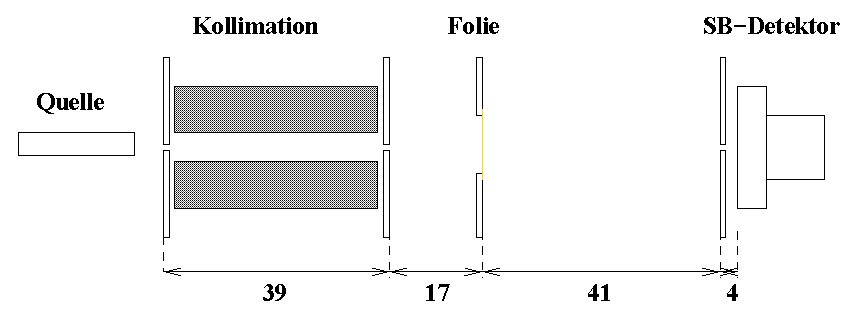
\includegraphics[width=0.7\textwidth]{content/grafik/Aufbau.pdf}
	\caption{Schematische Darstellung des verwendeten Versuchsaufbaus \cite{rutherford}.}
	\label{fig:Aufbau}
\end{figure}

\subsection*{Versuchsdurchführung}

Zu Beginn wird die Kammer evakuiert, um Ablenkungen der $\alpha$-Strahlung durch Luftmoleküle zu minimieren. Der Kammerdruck wird durch langsames Öffnen des Feindosierventils eingestellt.

Die Dicke der Streufolie wird durch Messung des Energieverlusts der Alphateilchen beim senkrechten Durchgang durch die Folie bestimmt. Die Impulshöhen der Detektorsignale werden bei unterschiedlichem Kammerdruck gemessen, sowohl mit als auch ohne Streufolie. Anschließend wird die Reichweite der Alphateilchen extrapoliert, um die Dicke der Folie zu berechnen.

Zur Untersuchung des differentiellen Wirkungsquerschnitts wird die Zählrate in Abhängigkeit vom Streuwinkel $\Theta$ gemessen. Der differentielle Wirkungsquerschnitt wird als Funktion des Streuwinkels aufgetragen und mit theoretischen Werten verglichen. 

